\documentclass{IEEEtran}

\usepackage{mathtools}
\usepackage{amsmath}
\usepackage{graphicx}
\usepackage{subfig}
\usepackage{verbatim}
\usepackage{algpseudocode}
\usepackage{natbib}
\usepackage{url}
\usepackage{listings}
\usepackage[spanish]{babel}
\usepackage[utf8x]{inputenc}
\usepackage{float}
\usepackage{array}
\usepackage{booktabs}
\usepackage{color}

%\setcounter{MaxMatrixCols}{16}

\begin{document}

\title{Informe Tarea 04}
\date {Junio de 2013}
\author{\IEEEauthorblockN{Tatiana Lopez Guevara \\}
\IEEEauthorblockA{Universidad Tecnológica de Pereira\\
tatiana@sirius.utp.edu.co }}
\maketitle


\begin{abstract}
El presente documento explica los resultados obtenidos en la implementación del algoritmo
de RANSAC para la estimación robusta de homografías. 
La implementación se realizó sobre OpenCV.
\end{abstract}

\begin{IEEEkeywords}
Computer Vision
\end{IEEEkeywords}

\section{Introducción}

Se empleó el algoritmo RANSAC para estimar una homografía entre 2 imágenes
que no se vea afectada por los outliers.

El número mínimo de correspondencias para calcular una homografía es de 4.
Según lo visto en clase, el valor recomendado de este parámetro para el 
algoritmo DLT es entre 4 y 6. Para esta implementación
se tomó un valor de 5.

Con respecto al valor de $p$ (probabilidad de que al menos un conjunto de
$n$ datos tomados al azar no contenga outliers), se escogió en un valor
de $99\%$

La entrada al programa implementado corresponde a la salida de las correspondencias
encontradas por el algoritmo NCC entre las esquinas de Harris de cada par de imágenes
de entrada realizado en la tarea 3. El resultado de estas correspondencias se 
carga desde un archivo (output de la tarea 3) con el siguiente formato:

\begin{verbatim}

N
X11 Y11 X12 Y12
...
X_N1 Y_N1 X_N2 Y_N2

\end{verbatim}

Donde N es la cantidad total de corresponencias encontradas
entre las esquinas $(X1_i, Y1_i)$ de la primera imágen con
las esquinas $(X2_i, Y2_i)$ de la segunda.

Las pruebas se realizaron sobre las 3 imágenes de prueba de la tarea 3.

\section{Ajuste del Modelo}
Para el ajuste del modelo se aplicó el método DLT - \textit{Direct Linera Transformation}
la cual busca minimizar el error de $A_i h =0$ \cite{hartley2000multiple}, donde:

\begin{equation*}
\begin{aligned}
\begin{pmatrix}
\vec{0}^T & -w'_i\vec{x}_i^T & y'_i \vec{x}_i^T \\ 
 w'_i\vec{x}_i^T & \vec{0}^T & -x'_i \vec{x}_i^T \\ 
 \end{pmatrix}_{2x9}
\left(
\begin{array}{c}
\vec{h}^1 \\
\vec{h}^2 \\
\vec{h}^3
 \end{array} 
 \right)_{9x1}
=
\vec{0}_{2x1}
\end{aligned}
\end{equation*} 

La solución a esta ecuación para el vector $\vec{h}$ está dada por la última columna
del vector $V$ en la descomposición de valor singular de $A$ en $U D V^T$.

\section{Concenso - Número de Inliers}

Una vez estimado el modelo con los datos de la muestra,
se procedió a calcular el error de transferencia simétrica \cite{hartley2000multiple},
el cual se tomó como criterio para determinar si una pareja
de correspondencias era inlier o no.

\begin{equation*}
\begin{aligned}
Err_{tsym} = \displaystyle\sum_i d(x_i, H^{-1}x'_i)^2 + d(x'_i, Hx_i)^2
\end{aligned}
\end{equation*} 

El valor del umbral dependía de la imágen sobre la cuál se estuviera
probando.
Estos valores se escogieron después de probar con
diferentes valores. Por ejemplo, para la imágen 1
se evaluaron los mostrados en el Cuadro \ref{tb:thrs1}
y figura \ref{fig:thrs1}.

\begin{table}[H]
\centering
\begin{tabular}{*2c}
\toprule
 Umbral & Inliers \\
 \midrule
0.10000&   17.00000\\
0.20000&   22.00000\\
0.30000&   24.00000\\
0.34000&   26.00000\\
{\color{red}0.35000}&   {\color{red}27.00000}\\
0.40000&   27.00000\\
0.50000&   27.00000\\
\bottomrule
 \end{tabular}
 \caption{Valores de Umbral para imágenes de prueba.}
 \label{tb:thrs1}
 \end{table} 

\begin{figure}[H]
\caption{Selección de Umbral Imágen 1}
\centering
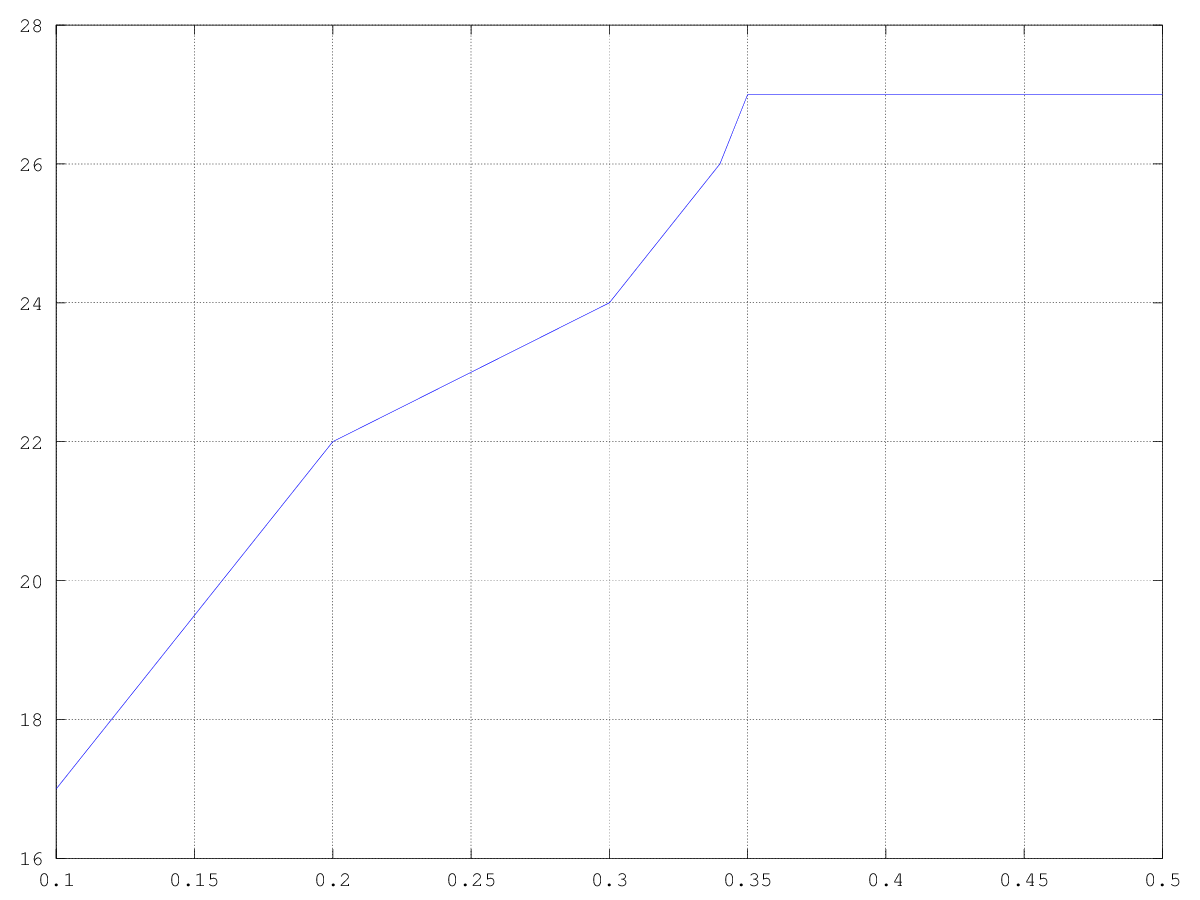
\includegraphics[width=6cm,natwidth=1200,natheight=900]{figs/thrs1.png}
\label{fig:thrs1}
\end{figure} 

A continuación se muestran los umbrales seleccionados para
las 3 imágenes de prueba después de realizar el proceso anteriormente
mencionado con todas. Adicionalmente se muestra la cantidad total de correspondencias
y la cantidad de inliers/outliers detectados para dichos umbrales.

\begin{table}[H]
\centering
\begin{tabular}{*5c}
\toprule
 & Umbral & ntot & Inliers &Outliers \\
\midrule
Imágen 1 & 28 &  0.35f & 27 & 1\\
Imágen 2 & 71 & 4.0f & 43 & 28\\
Imágen 3 & 900.0f & 519 & 292 & 227\\
\bottomrule
\end{tabular}
\caption{Valores de Umbral para imágenes de prueba.}
\label{tb:umbral}
\end{table} 

\section{Colinealidad}

La verificación de colinealidad entre los 5 puntos seleccionados
aleatoriamente se realizó para todos los conjuntos de 3 puntos
que se pudieran armar:

\begin{equation*}
\begin{aligned}
\binom{5}{3} = 10
\end{aligned}
\end{equation*} 

Sean p1, p2 y p3 los puntos a evaluar. La colinealidad se verificó
mediante:

\begin{equation*}
\begin{aligned}
l &= p1 \times p2 \\
&p3'l \stackrel{?}{\approx} \epsilon
\end{aligned}
\end{equation*} 

\section{Resultados RANSAC}

En la gráfica \ref{fig:bigimg_1} se muestra el resultado
obtenido por RANSAC una vez se reestimó el modelo $(H)$
a partir del mejor set de inliers obtenido para la 
primera imágen de prueba.
En rojo se pueden apreciar las correspondencias que fueron
tomadas como outliers y en verde las que se tomaron como
inliers.

\begin{figure}[H]
\caption{Ilustración de los inliers (verde) y los outliers (rojo) para la Imágen 1}
\centering
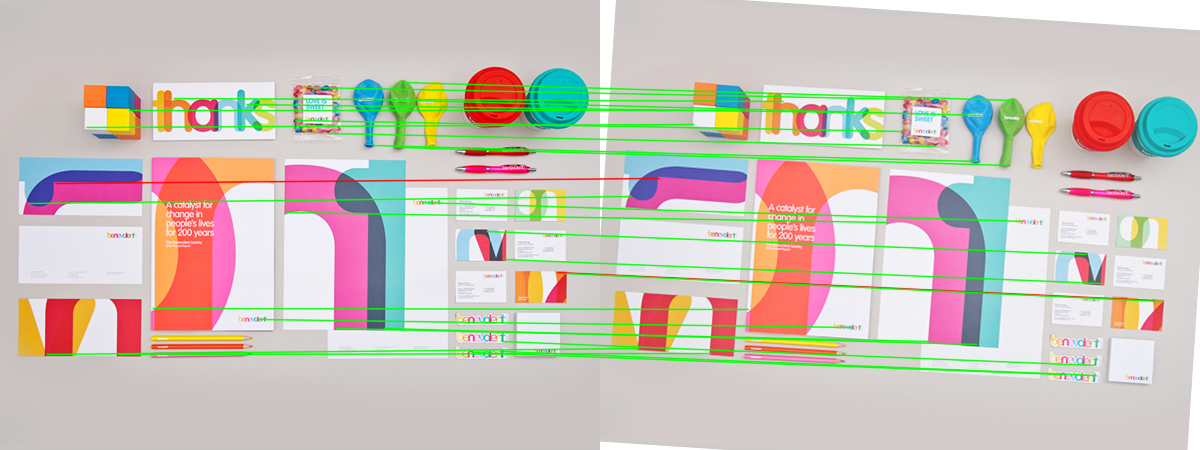
\includegraphics[width=9.5cm,natwidth=1200,natheight=450]{figs/bigimg_1.png}
\label{fig:bigimg_1}
\end{figure}

En la figura \ref{fig:img2_1} se muestra en amarillo las esquinas 
encontradas por Harris sobre la parte 2 de la imágen $(x')$ 
y en verde (inliers) y rojo (outliers) las proyecciones de las esquinas de la parte 1 mediante
la homografía encontrada por RANSAC $(Hx)$. Es decir, los amarillos son los datos
reales y los verdes y rojos, los proyectados mediante el H encontrado.

\begin{figure}[H]
\caption{Proyección de esquinas con la homografía encontrada $Hx, x'$ para la Imágen 1}
\centering

\includegraphics[width=8cm,natwidth=600,natheight=450]{figs/img2_1.png}
\label{fig:img2_1}
\end{figure}

En la figura \ref{fig:img1_1} se muestra el mismo procedimiento sobre
la primera parte de la imágen: $(x)$ y $(H^{-1}x')$.

\begin{figure}[H]
\caption{Proyección de esquinas con la homografía encontrada $H^{-1}x', x$ para la Imágen 1}
\centering

\includegraphics[width=8cm,natwidth=600,natheight=450]{figs/img1_1.png}
\label{fig:img1_1}
\end{figure}

\section{Otras Pruebas}

Los resultados obtenidos por el algoritmo para la imágen de prueba 2
de la tarea 3 se pueden apreciar en las figuras \ref{fig:bigimg_2}, 
\ref{fig:img2_2} y \ref{fig:img1_2}.

\begin{figure}[H]
\caption{Ilustración de los inliers (verde) y los outliers (rojo) para la Imágen 2}
\centering
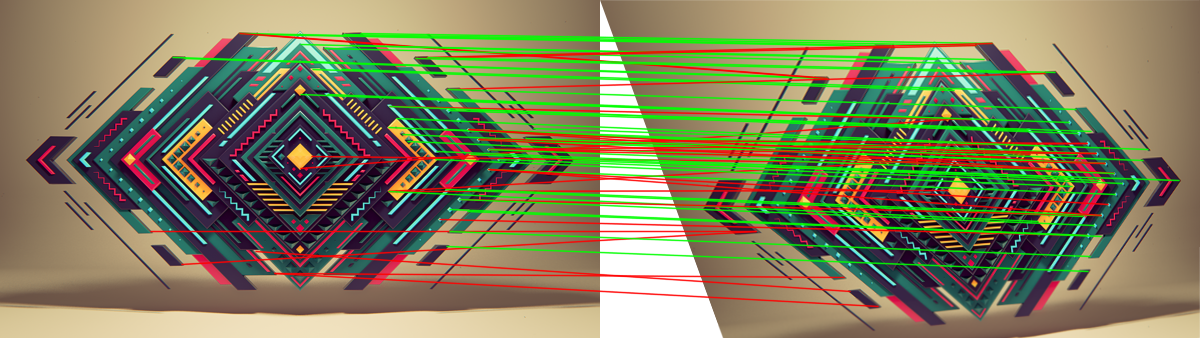
\includegraphics[width=9cm,natwidth=1200,natheight=450]{figs/bigimg_2.png}
\label{fig:bigimg_2}
\end{figure}

\begin{figure}[H]
\caption{Proyección de esquinas con la homografía encontrada $Hx, x'$ para la Imágen 2}
\centering
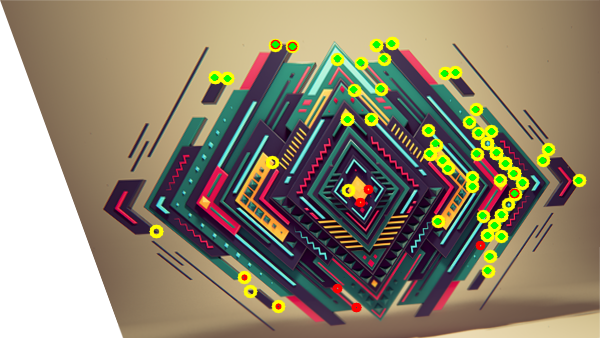
\includegraphics[width=8cm,natwidth=600,natheight=450]{figs/img2_2.png}
\label{fig:img2_2}
\end{figure}

\begin{figure}[H]
\caption{Proyección de esquinas con la homografía encontrada $H^{-1}x', x$ para la Imágen 2}
\centering
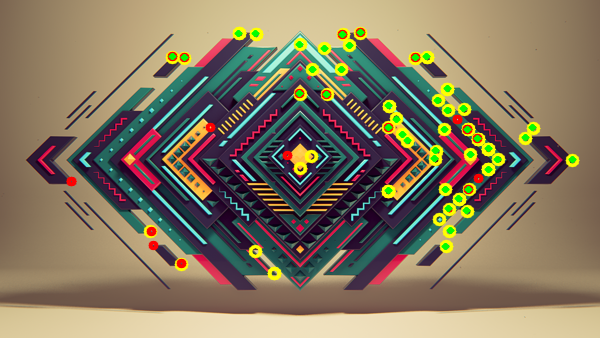
\includegraphics[width=8cm,natwidth=600,natheight=450]{figs/img1_2.png}
\label{fig:img1_2}
\end{figure}

En los resultados obtenidos por el algoritmo para la imágen de prueba 3
de la tarea 3 se puede apreciar que a pesar de que
las correspondencias detectadas como inliers en efecto sí corresponden 
(figura \ref{fig:bigimg_3}), la homografía encontrada no mapea exactamente
los puntos de $(Hx)$ sobre los de $(x')$ (figura \ref{fig:img1_3}) y viceversa
(figura \ref{fig:img2_3}).
Esto se alcanza a distinguir mejor en en jarrón de la parte superior izquierda
de la imágen, donde los puntos verdes correspondientes a la proyección 
están desplazados con respecto a los círculos amarillos.

Esto probablemente se deba a que ambas partes de la imágen fueron tomadas con
una cámara real y están sujetas no solo a la traslación, rotación y cambio de
luminosidad, sino a ruido. Esto contrasta con las otras 2 imágenes de prueba
mostradas anteriormente, las cuales son generadas digitalmente y cuya 
parte 2 fue generada aplicando una distorción concreta (rotación, perspectiva)
mediante Gimp.

\begin{figure}[H]
\caption{Ilustración de los inliers (verde) y los outliers (rojo) para la Imágen 3}
\centering
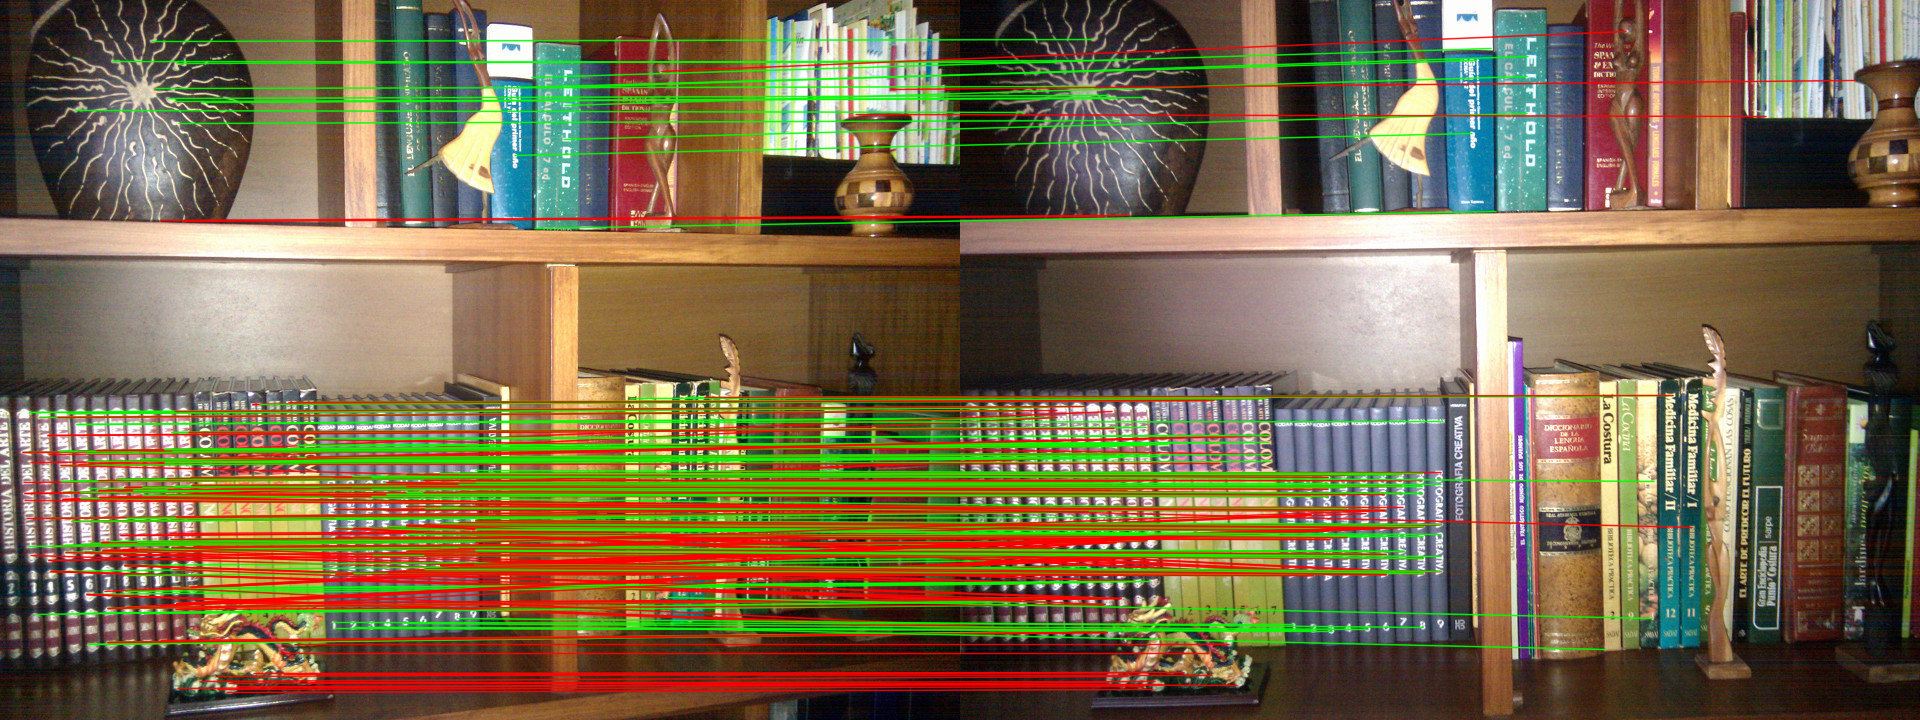
\includegraphics[width=9cm,natwidth=1200,natheight=450]{figs/bigimg_3.png}
\label{fig:bigimg_3}
\end{figure}

\begin{figure}[H]
\caption{Proyección de esquinas con la homografía encontrada $Hx, x'$ para la Imágen 3}
\centering
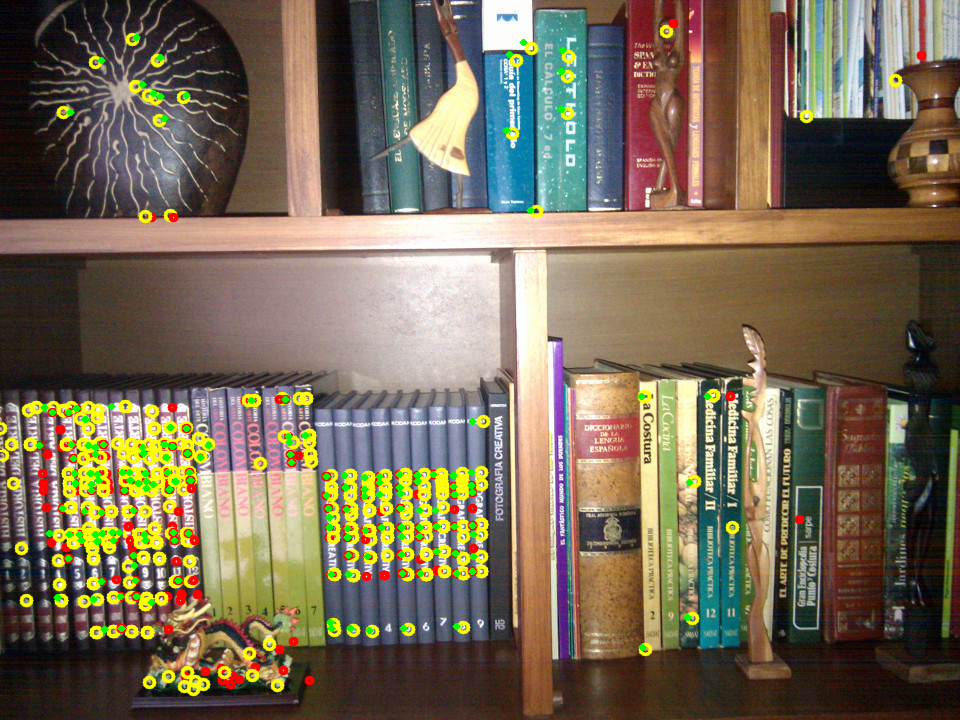
\includegraphics[width=8cm,natwidth=600,natheight=450]{figs/img2_3.png}
\label{fig:img2_3}
\end{figure}

\begin{figure}[H]
\caption{Proyección de esquinas con la homografía encontrada $H^{-1}x', x$ para la Imágen 3}
\centering
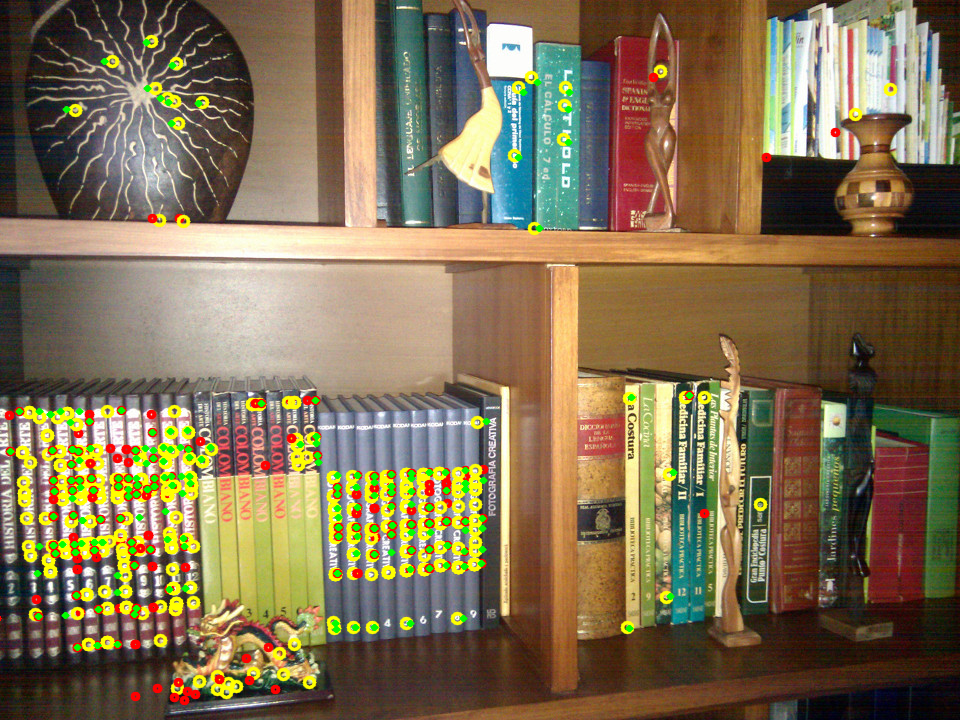
\includegraphics[width=8cm,natwidth=600,natheight=450]{figs/img1_3.png}
\label{fig:img1_3}
\end{figure}

En esta última prueba especialmente, se nota la necesidad de refinar la
homografía hallada mediante técnicas de minimización no lineal de 
mínimos cuadrados.

\section{DLT sobre todos los datos}

En la figura \ref{fig:DLT1} se muestra el resultado obtenido mediante
DLT sobre todos los pares de correspondencias, es decir, sin emplear RANSAC.
Se puede observar que los outliers afectan en gran medida el modelo en contraste
con el obtenido en la figura \ref{fig:img2_2} que sí emplea RANSAC para la
estimación.

\begin{figure}[H]
\caption{Proyección de esquinas con la homografía encontrada teniendo
en cuenta outliers $Hx, x'$ para la Imágen 2}
\centering
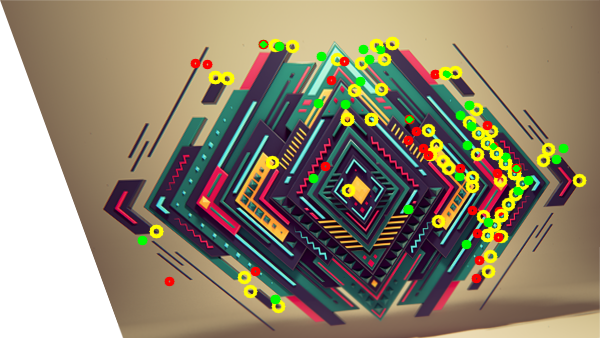
\includegraphics[width=8cm,natwidth=600,natheight=450]{figs/DLT1.png}
\label{fig:DLT1}
\end{figure}


Se empleó la imágen de prueba 2 ya que la primera no contiene outliers y por
lo tanto genera un resultado muy similar al de RANSAC.

\section{Ejecución}
Para la compliación del programa ejecutar:
\begin{verbatim}
make
\end{verbatim}

El modo de uso es:
\begin{verbatim}
./Ransac PathImg1 PathImg2 
         PathCorrespondencesFile threshold
\end{verbatim}

Para ejecutar con los valores por defecto (imágen de prueba 1), 
simplemente ejecute:
\begin{verbatim}
./Ransac
\end{verbatim}

Para ejecutar las pruebas mostradas en este informe, 
ver el archvo \verb+README.txt+.

\section{Conclusiones}
\begin{itemize}
\item El algoritmo de RANSAC converge de forma 
muy rápida comparado con el total de posibilidades
que se deberían evaluar mediante fuerza bruta
$\binom{N}{5}$.
\item El valor del umbral para determinar si un dato 
es inlier o no varía mucho de una imágen a otra debido
a que la varianza del ruido es un valor intrínseco
de la imágen tomada. Esto se nota especialmente en la
imágen de prueba 3 cuyas 2 partes fueron tomadas con
una cámara real.
\item La homografía estimada a partir de imágenes digitales 
sobre las que se ha aplicado alguna distorción mediante 
un programa de edición de imágenes, presentó una aproximación\
casi perfecta de los datos. Sin embargo, la homografía econtrada
para 2 fotografías tomadas con una cámara generó una homografía
donde los puntos transformados están situados a una distancia $d$
de los puntos reales. En este caso, es necesario refinarlo
mediante técnicas de estimación robusta como Levenverg-Marquardt.
\end{itemize} 

\bibliographystyle{plain}
\bibliography{biblio}

\end{document}
